\documentclass[conference]{IEEEtran}
\IEEEoverridecommandlockouts
% The preceding line is only needed to identify funding in the first footnote. If that is unneeded, please comment it out.
\usepackage{cite}
\usepackage{amsmath,amssymb,amsfonts}
\usepackage{algorithmic}
\usepackage{graphicx}
\usepackage{textcomp}
\usepackage{xcolor}
\def\BibTeX{{\rm B\kern-.05em{\sc i\kern-.025em b}\kern-.08emT\kern-.1667em\lower.7ex\hbox{E}\kern-.125emX}}
\begin{document}
\title{Machine Learning\\
{\footnotesize \textsuperscript{*}Analyzing problems, designing a machine learning solution, implementing ML algorithms, and evaluating  data sets }
}

\author{\IEEEauthorblockN{1\textsuperscript{st} Saksham Saxena}
\IEEEauthorblockA{\textit{dept. name of organization (of Aff.)} \\
\textit{name of organization (of Aff.)}\\
City, Country \\
email address}
\and
\IEEEauthorblockN{2\textsuperscript{nd} Rushabh Doshi}
\IEEEauthorblockA{\textit{dept. name of organization (of Aff.)} \\
\textit{name of organization (of Aff.)}\\
City, Country \\
email address}
\and
\IEEEauthorblockN{3\textsuperscript{rd} Luke Beaulieu}
\IEEEauthorblockA{\textit{dept. name of organization (of Aff.)} \\
\textit{name of organization (of Aff.)}\\
City, Country \\
email address}
\and
\IEEEauthorblockN{4\textsuperscript{th} Utkarsh Patel}
\IEEEauthorblockA{\textit{dept. name of organization (of Aff.)} \\
\textit{name of organization (of Aff.)}\\
City, Country \\
email address}
}

\maketitle


\begin{abstract}
This paper presents the analysis and evaluation on data sets using machine learning techniques. Our method in this assignment consist of working with three data sets and implement ML algorithms on them to understand more about the field of machine learning and its applications in the real world. The three three data sets worked on in this project was  Boston housing, breast cancer, and Forest Covertype.
\end{abstract}

\begin{IEEEkeywords}
introduction, methodology, result, discussion, conclusion
\end{IEEEkeywords}

\section{Introduction}
The goal of this final project is to show that we have learned something in the class. It is an opportunity for us to explore ideas that we have see in the lectures and assignments and extend them. This project is a first steps towards research in machine learning or its applications. We will analyze problems, design a machine learning solution, implement ML algorithms, and evaluate them on three data sets (one for classification and one for regression from “Small Data Sets” and one data set – either classification or regression – from “Large Data Sets”).

\section{Problem and Data sets}
\subsection{Breast Cancer, logistic regression}\label{AA}
Breast cancer data set is a classification data set. The output variable of the cancer data was either malignant or benign .
%○ What are the important ideas/methods you explored?
%○ What ideas from the class did you use?
%○ Reporting the results (cross-validation, easy-to-read figures, etc)
%○ Do the results make sense?
%○ If you had much more time, how would you continue the project?

\begin{figure}[htbp]
\centerline{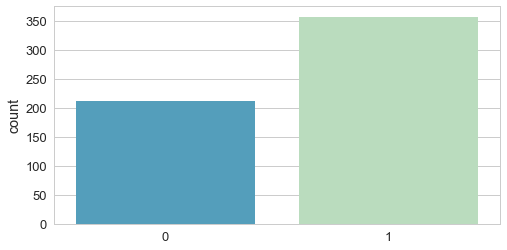
\includegraphics[width=50mm,scale=0.5]{imgs/output_16_1.png}}
\caption{0: Malignant 1: Benign}
\label{fig}
\end{figure}

Since this is a classification data set, it was important to go back and look at which methods I could and could not use to work with this data set. I chose logistic regression model in this case. The idea of logistic regression is that there is an optimal decision boundary that separates the two classes of cancer. From class, we learned methods to obtain that optimal decision boundary using cost function.

For the given training data, we want to find parameters $\Theta$ that are most likely by maximizing L($\Theta$). This is the maximum likelihood estimator.
\begin{figure}[htbp]
\centerline{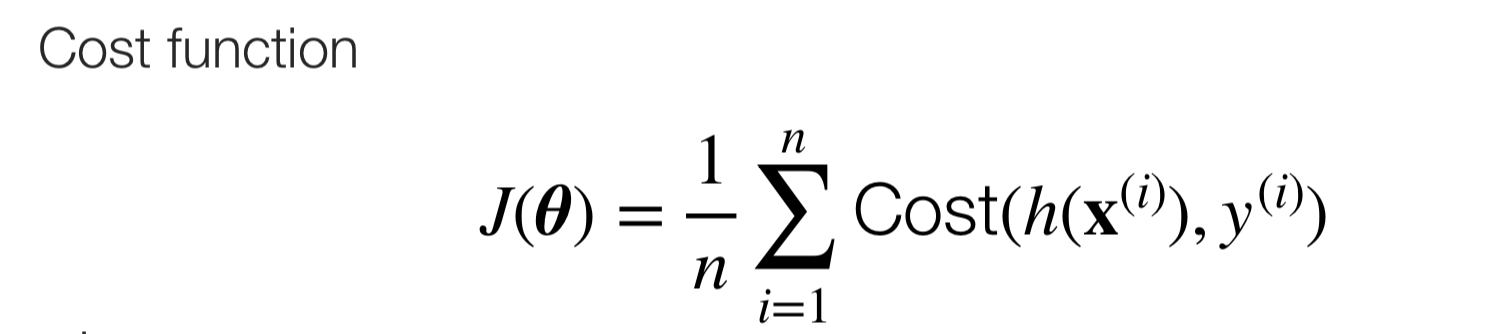
\includegraphics[width=50mm,scale=0.5]{imgs/cost_func}}
\label{fig}
\end{figure}

\begin{figure}[htbp]
\centerline{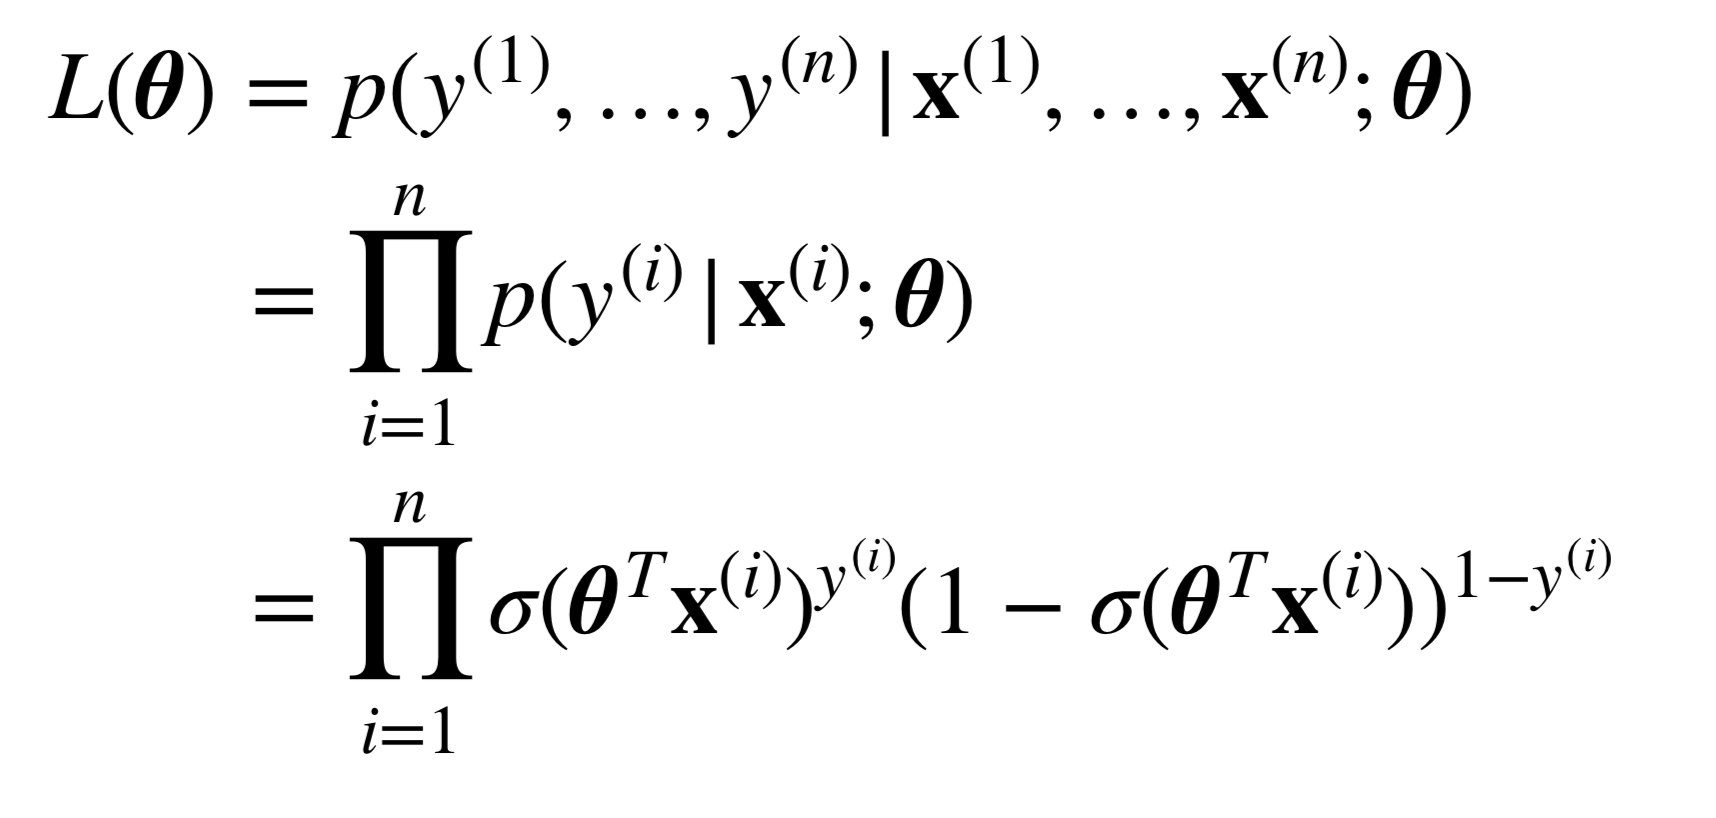
\includegraphics[width=50mm,scale=0.5]{imgs/max_like}}
\caption{maximum likelihood estimator function}
\label{fig}
\end{figure}
Knowing the likelihood function (above) for this given problem, we look for such $\Theta$ that maximizes the probability of obtaining the data we have. To find the $\Theta$, we have an optimization algorithm to find that $\Theta$.
\begin{figure}[htbp]
\centerline{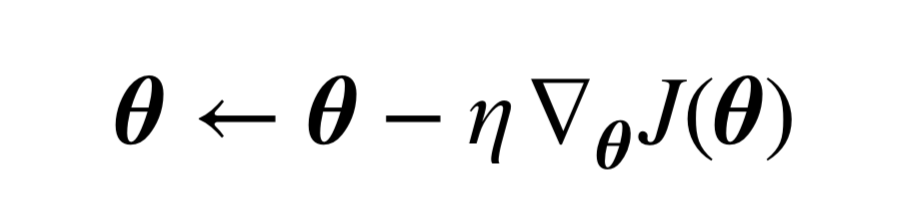
\includegraphics[width=50mm,scale=0.5]{imgs/gradient}}
\caption{gradient descend where n is the learning rate }
\label{fig}
\end{figure}
\newpage
Going through different learning rates and iterations, this leaves us with an optimal line that separates the two classification of breast cancer. *n is the learning rate and it determines how big of a step we get to the minimum point in the gradient descend.  
\noindent-Too big of a learning rate causes drastic updates which leads to divergent behavior. 
\noindent-Too small of a learning rate and it may take a lot of iterations to get to the minimum point. 
\begin{figure}[htbp]
\centerline{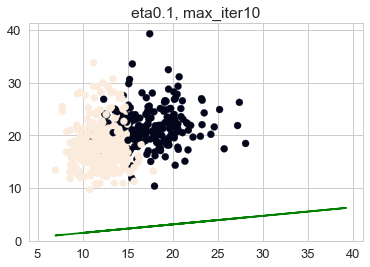
\includegraphics[width=50mm,scale=0.5]{imgs/output_20_1.png}}
\caption{Small learning rate and iteration}
\label{fig}
\end{figure}
\begin{figure}[htbp]
\centerline{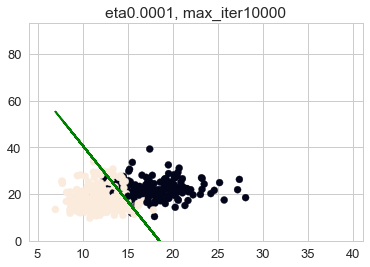
\includegraphics[width=50mm,scale=0.5]{imgs/output_20_16.png}}
\caption{Good learning rate and iteration}
\label{fig}
\end{figure}

Although I did not have enough time to find the numerical of the errors and accuracy, that is what I would have liked to do if i had more time.(doable using train  and test using a 40:60 split model)

The logistic model optimally draws the line between two classes of data, so these results (graphs) do make sense.

%%%%%%%%%%%%%%%%%%%%%%%%%%%%%%%%%%%%%%%%%%%%%%%%%%%%%%%%%%%%%%%%%%%%%%%%%%%%%%%%%%%%%%%%%%%%%%%%%%%%%%%%%%%%%%%%%%%%%%%%%%%%%%%%%%%%%%%%%%%%%%%%%%%%%%%%%%%%%%%%%%%%%%%%%%%%%%%%%%%%%%%%%%%%

\subsection{Breast Cancer, Support Vector Machine}
%○ What are the important ideas/methods you explored?
%○ What ideas from the class did you use?
%○ Reporting the results (cross-validation, easy-to-read figures, etc)
%○ Do the results make sense?
%○ If you had much more time, how would you continue the project?
Support Vector Machine or SVM is another method for classification problems such at breast cancer. This works efficiently on datasets that are linearly separable, and so what SVM attempts to do is separate the data by a 'separating hyperplane'.  An SVM model is a representation of the examples as points in space, mapped so that the examples of the separate categories are divided by a clear gap that is as wide as possible. New examples are then mapped into that same space and predicted to belong to a category based on which side of the gap they fall. [wiki].

The methodology for SVM was to setup the data frame and use a train test 40:60 split. Then using the support vector classifier, or SVC model, I went to predict the accuracy of the model, how well it maps new data or examples for this data. 

\newpage
\begin{figure}[htbp]
\centerline{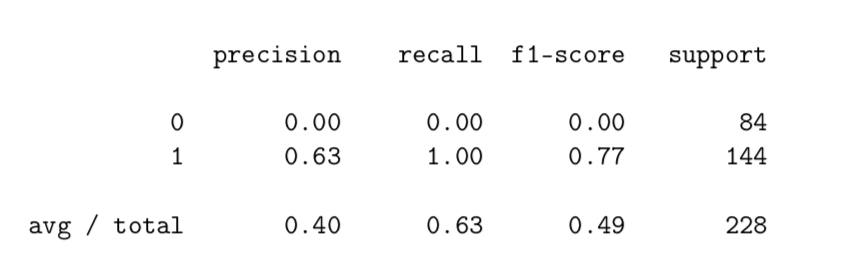
\includegraphics[width=50mm,scale=0.5]{imgs/class1}}
\caption{Prediction with no adjustment}
\label{fig}
\end{figure}
Obviously this was not a good prediction without training, adjustment, and normalizing the data. The model is fairly inaccurate. 

For the parameters of the SVC model, we want to use \textbf{grid search} to find the best parameter, specifically C and $\Gamma$. Grid search runs the same loop with cross-validations to find the best parameters. Once it has found the best combinations, it runs fit on all the data passed to build a single model using the best parameter setting.

\begin{figure}[htbp]
\centerline{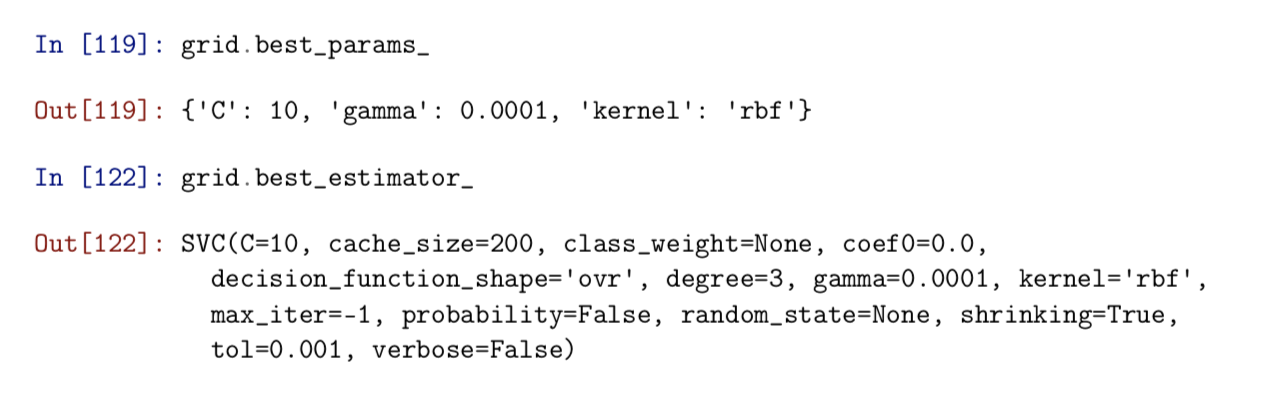
\includegraphics[width=50mm,scale=0.5]{imgs/params}}
\caption{best parameters \& estimator}
\label{fig}
\end{figure}

You can pull out the best parameters and estimators from grid search. With the adjusted parameters and normalization of the train test split data, we get a better accuracy for the model.

\begin{figure}[htbp]
\centerline{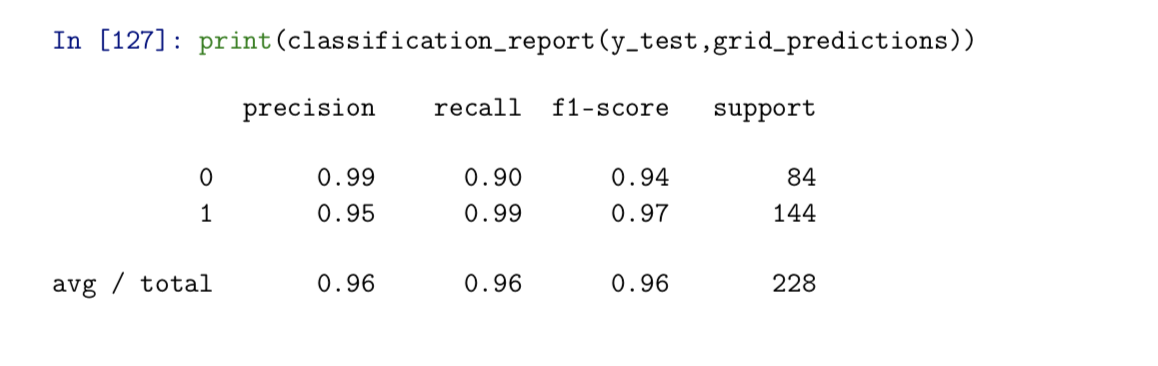
\includegraphics[width=50mm,scale=0.5]{imgs/class2}}
\caption{Prediction with  adjustment + normalization}
\label{fig}
\end{figure}

The SVC model does make sense in terms of mapping an example to a class with an accuracy of 96\%. With more time, I would extend this project to set up more classification models, including Neural Networks and K-Mean Clustering. With these different models, an obvious thing to do is compare and contrast the different models. An entire different report on the comparison would include errors margins, efficient margins and more data to describe the different techniques used. 

On the side, this project could extend to doing research and problem solving in other areas aside from the data sets we worked on. I would have loved to do a research project on how students past grades affect future classes, but that is for the future and a different time.

%%%%%%%%%%%%%%%%%%%%%%%%%%%%%%%%%%%%%%%%%%%%%%%%%%%%%%%%%%%%%%%%%%%%%%%%%%%%%%%%%%%%%%%%%%%%%%%%%%%%%%%%%%%%%%%%%%%%%%%%%%%%%%%%%%%%%%%%%%%%%%%%%%%%%%%%%%%%%%%%%%%%%%%%%%%%%%%%%%%%%%%%%%%%

\subsection{Boston Housing , linear regression}
%○ What are the important ideas/methods you explored?
%○ What ideas from the class did you use?
%○ Reporting the results (cross-validation, easy-to-read figures, etc)
%○ Do the results make sense?
%○ If you had much more time, how would you continue the project?
The Housing dataset contains information about houses in Boston but the information is from early 1990’s. The dataset is available in the scikit learn library. It contains 506 samples and 13 feature sets including features like number of rooms, age of the house and per capita crime rate of the town. The objective is to predict the price based on the price data available for the given samples.

\begin{figure}[htbp]
\centerline{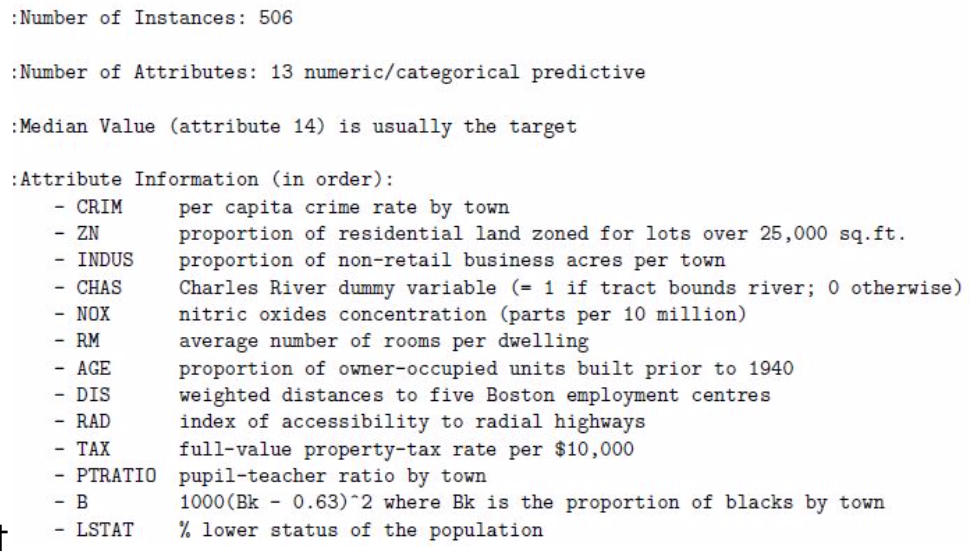
\includegraphics[width=50mm,scale=0.5]{imgs/analysis1}}
\label{fig}
\end{figure}

 We started with analyzing the dataset to get a better understanding of the data before us. To get more information about the features, we used boston.DESCR function to get a detailed information about each of the feature. Before using the data, it’s always a good habit to preprocess the data and look for some missing values. Fortunately, there wasn’t any missing value in our dataset. Next, we used the heatmap function of seaborn library to get the correlation matrix that measures the linear relationship of each feature with our target value as well as with all other features. 
 
\begin{figure}[htbp]
\centerline{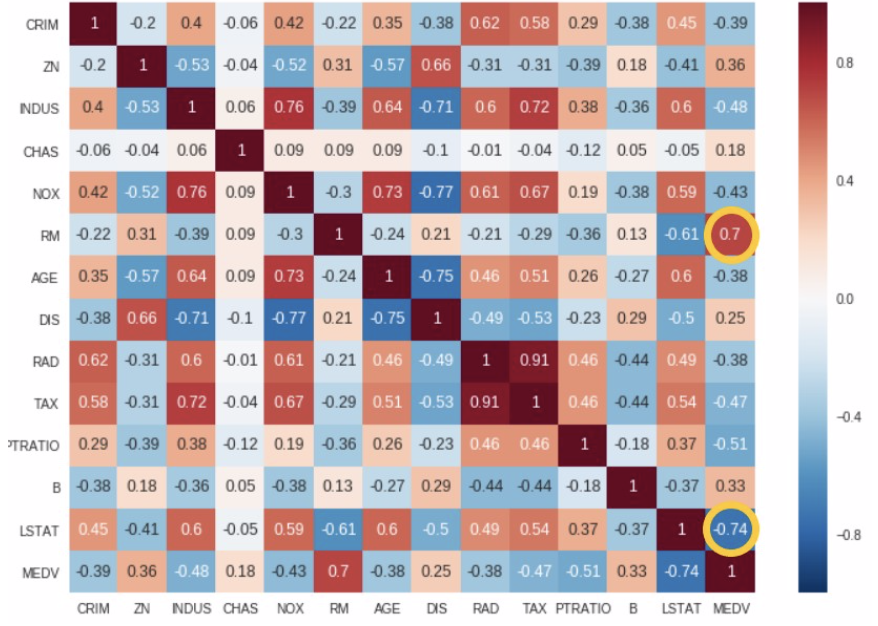
\includegraphics[width=50mm,scale=0.5]{imgs/heatmap}}
\label{fig}
\end{figure}

To fit a linear regression model, we selected those features which have a high correlation with our target variable MEDV(Price). By looking at the correlation matrix we can see that RM has a strong positive correlation with MEDV(0.7) where as LSTAT has a high negative correlation with MEDV(-0.74). The important thing to keep in mind here is to avoid those features with multi-co-linearity. As can be seen in the heatmap image, RAD and TAX have a correlation of 0.91. Let’s consider an example to understand why we do so. Consider the simplest case where Y is regressed against X and Z and where X and Z are highly positively correlated. Then the effect of X on Y is hard to distinguish from the effect of Z on Y because any increase in X tends to be associated with an increase in Z. So based on these observations, we used RM and LSTAT as our features to build the Linear Regression model. 

\begin{figure}[htbp]
\centerline{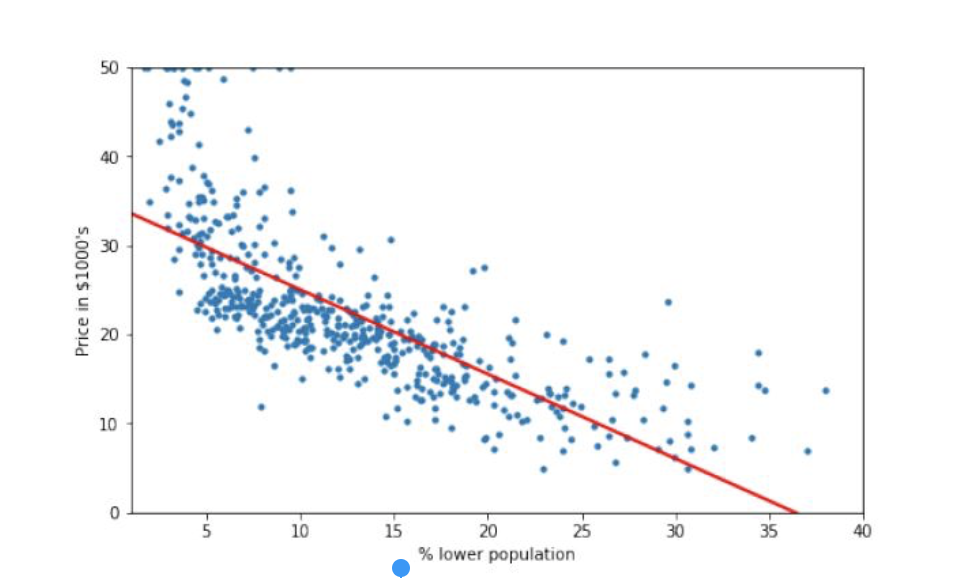
\includegraphics[width=50mm,scale=0.5]{imgs/img1}}
\label{fig}
\end{figure}

\begin{figure}[htbp]
\centerline{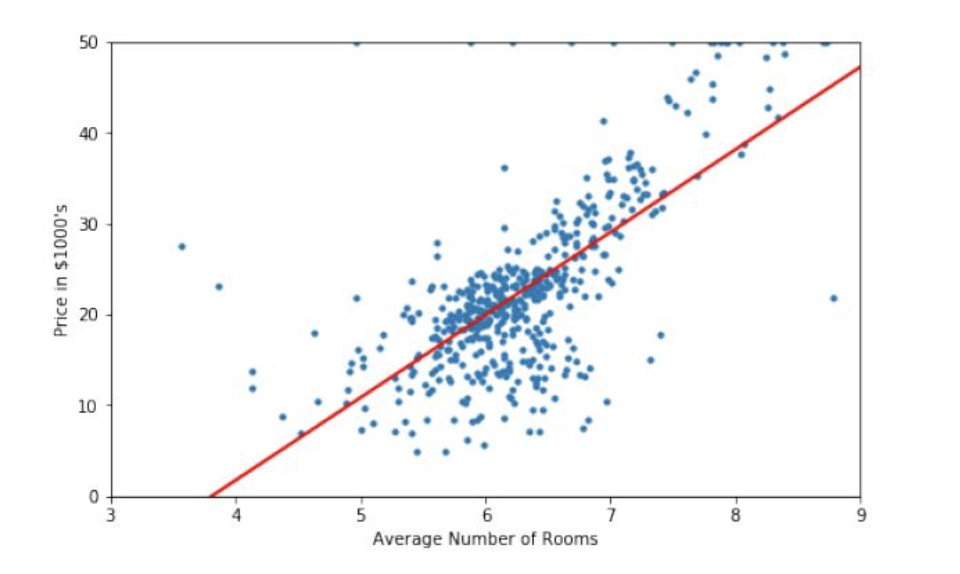
\includegraphics[width=50mm,scale=0.5]{imgs/img2}}
\label{fig}
\end{figure}

At this point, I ran an experiment to check whether the linear model improves based on my assumptions or not. I built the Linear Regression model using the scikit learn class. But instead of one, I made two models and compared the results. In the first model, I just selected the two features which we got from analyzing the data before. In the second model, I selected all the 13 features to see whether it has any effect on the predictions. Even though I did get a better result based on RMSE for the first model, the difference in the RMSE values wasn’t as big as I expected it to be. And this is something which I need to think about and try to understand the reasoning behind it.



%%%%%%%%%%%%%%%%%%%%%%%%%%%%%%%%%%%%%%%%%%%%%%%%%%%%%%%%%%%%%%%%%%%%%%%%%%%%%%%%%%%%%%%%%%%%%%%%%%%%%%%%%%%%%%%%%%%%%%%%%%%%%%%%%%%%%%%%%%%%%%%%%%%%%%%%%%%%%%%%%%%%%%%%%%%%%%%%%%%%%%%%%%%%

\subsection{Forest Covertype}
\noindent \textbf{Dataset}

\noindent The complete dataset is composed by 581,012 instances, where each observation (instance) corresponds to a 30 x 30 meters cell. For each observation, 12 measures (attributes) are given. However, two categorical properties (wilderness area and soil type) were binarized, in order to have a dataset composed only by numerical attributes. So, the final dataset is composed by 10 quantitative variables, 4 binary wilderness areas and 40 binary soil type variables, given a total of 54 columns of data. Below, some description about these attributes is given:
\begin{itemize}
\item{Elevation: Elevation in meters.}
\item{Aspect: Aspect in degrees azimuth. }
\item{Slope: Slope in degrees.}
\item{Horizontal distance to hydrology: Horizontal distance to nearest surface water features. }
\item{Vertical distance to hydrology: Vertical distance to nearest surface water features. }
\item{Horizontal distance to roadways: Horizontal distance to nearest roadway. }
\item{Hillshade 9am: Hillshade index at 9am, summer solstice (0 to 255). }
\item{Hillshade Noon: Hillshade index at noon, summer soltice (0 to 255). }
\item{Hillshade 3pm: Hillshade index at 3pm, summer solstice (0 to 255). }
\item{Horizontal distance to fire points: Horizontal distance to nearest wildfire ignition points. }
\item{Wilderness area: Wilderness area designation. 4 binary columns, 0 (absence) or 1 (presence). }
\item{Soil type: Soil type designation. 40 binary columns, 0 (absence) or 1 (presence). }
\item{Cover Type: Forest cover type designation. This is the attribute to be predicted (1 to 7).}
\end{itemize}

Regarding the Cover Type attribute, the following distribution is observed in the whole dataset:
\begin{figure}[htbp]
\centerline{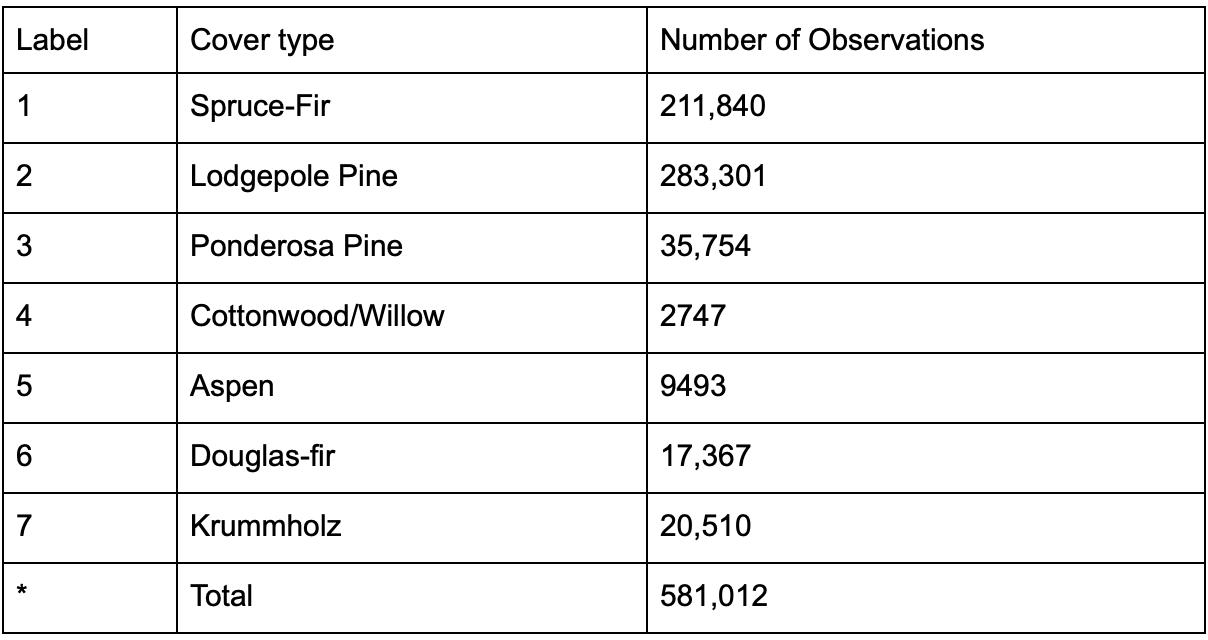
\includegraphics[width=50mm,scale=0.5]{imgs/dataset_table}}
\label{fig}
\end{figure}

\noindent \textbf{Random Forest}

\noindent A random forest is a meta estimator that fits a number of decision tree classifiers on various sub-samples of the dataset and use averaging to improve the predictive accuracy and control over-fitting. We use sklearn.ensemble. RandomForestClassifier from scikit-learn package to do the classification. 

\noindent ensemble.RandomForestClassifier(n\_estimator = 100, max\_depth = 2, random\_state = 0)
n\_estimators stands for the number of trees in the forest.
We use fit(X, y) to build a forest of trees from the training set (X, y) and predict(X) to predict class for X.
Stratified Dataset
Another method that was used was stratifying the dataset. When a dataset is very highly skewed with a particular label field. It can affect the performance of that model, because the dataset the model was trained on is not reflective of the dataset the model was tested on. When a dataset is stratified, the dataset is split in a way where the class distribution of the train dataset is roughly equal to the test dataset. 

\noindent \textbf{Concepts from class}

\noindent One technique taught in class that was implemented in this project was normalization. With the tree cover dataset, the data varies from measurements in meters to boolean values. By normalizing the dataset you ensure that the model takes into account the values in reference to other values in the same feature. Rather 
than in reference to the other features.

\begin{figure}[htbp]
\centerline{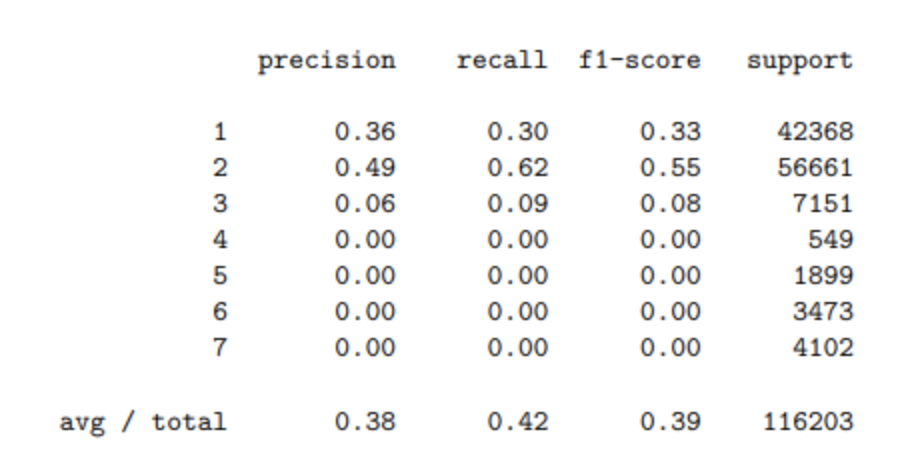
\includegraphics[width=50mm,scale=0.5]{imgs/class_report}}
\caption{classification report}
\label{fig}
\end{figure}

\begin{figure}[htbp]
\centerline{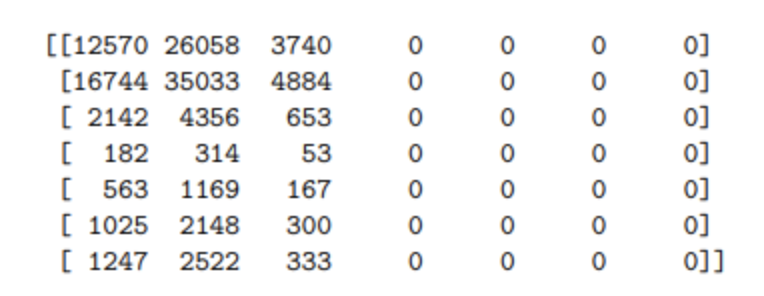
\includegraphics[width=50mm,scale=0.5]{imgs/conf_matrix}}
\caption{confusion matrix}
\label{fig}
\end{figure}

\noindent \textbf{Analyzing Results}

\noindent  Regardless of normalization, feature selection, number of epochs, or hidden layer shape, the model consistently performed between 39\% and 42\% regardless of stratification. There seems to not be enough of a distinction between each class of trees because the model at its best performance appears to just guess randomly based of the expected distribution. 

\noindent \textbf{More Time}

\noindent If I had more time I would try to look into whether or not there are other datasets for different areas which have similar data. I would train a model on the other dataset to see if the model has improved results, because I think that the dataset is the real problem. That is why there is no variation based on model changes. Once I have improved the data, I would run a optimization algorithm which would vary hidden layer shape, steps, and epochs. Run several tests for each instance, average the results, then record the best performing values.




\end{document}
